\documentclass[hyperref={pdfpagelabels=false},aspectratio=34,14pt]{beamer}
\usepackage{lmodern} %TODO: descobrir o que mudou as fontes dos slides (comparar com os primeiros)
\usepackage[utf8]{inputenc}
\usepackage[T1]{fontenc}
\usefonttheme[onlymath]{serif}
\usepackage[brazil]{babel}
\usepackage[outputdir=..]{minted}
\usepackage{xcolor}
\usepackage{soul} % strikethrough
\usepackage{advdate}
\usepackage{graphicx}
\usepackage[ampersand]{easylist}
\usepackage{multirow}
\usepackage{tikz}
\usetikzlibrary{shapes,arrows,positioning}
\usetikzlibrary{circuits.logic.US}
\usetikzlibrary{matrix,calc}
\usepackage{karnaugh-map}

\usepackage{pgfpages}
\setbeamertemplate{note page}{\pagecolor{yellow!5}\insertnote}\usepackage{palatino}
\newcommand{\yes}{edge node [above] {yes}}
\newcommand{\no}{edge  node [left]  {no}}
\newcommand{\textttb}[1]{\textcolor{blue}{\ttfamily #1}}

% \setmathfont{Latin Modern Math}[version=lm]

\graphicspath{{../figs/}}

\definecolor{bgc}{rgb}{0.95,0.9,0.95}
\definecolor{links}{HTML}{2A7F7F}
\hypersetup{colorlinks,linkcolor=,urlcolor=links}

\newminted{verilog}{fontsize=\scriptsize, 
		   linenos,
		   numbersep=8pt,
           bgcolor=bgc,
           tabsize=4,
		   framesep=3mm} 
%		   frame=lines,

\newcommand{\verilog}[1]{\verilogf{#1}{\footnotesize}

\newcommand{\verilogf}[2]{\inputminted[fontsize=#2, 
		   linenos,
		   tabsize=2,
		   numbersep=4pt,
           bgcolor=bgc,
		   framesep=3mm]{verilog}{../codes/#1.v}
}

\newminted{nasm}{fontsize=\scriptsize, 
		   linenos,
		   numbersep=8pt,
           bgcolor=bgc,
		   framesep=3mm} 

% \author[shortname]{\scriptsize Prof. Edilson Kato \and Prof. Maurício Figueiredo \and Prof. Ricardo Menotti\newline
% \href{mailto:kato@ufscar.br}{kato@ufscar.br} \and    \href{mailto:mauricio@ufscar.br}{mauricio@ufscar.br} \and
% \href{mailto:menotti@ufscar.br}{menotti@ufscar.br}}

\newcommand{\newauthor}[2]{
  \parbox{0.40\textwidth}{
    \texorpdfstring
      {
        \centering
        \footnotesize #1 \newline
        {\scriptsize{\urlstyle{same}\href{mailto:#2}{#2}\urlstyle{tt}}}
      }
      {#1} \newline
  }
}

\author{
%   \newauthor{Prof. Edilson Kato}{kato@ufscar.br}
% \and
  \newauthor{Prof. Ricardo Menotti}{menotti@ufscar.br}
\and 
  \newauthor{Prof. Maurício Figueiredo}{mauricio@ufscar.br}
% \and
%   \newauthor{Prof. Roberto Inoue}{rsinoue@ufscar.br}
}

\institute{\href{http://www.dc.ufscar.br/}{Departamento de Computação} \\
           \href{http://www.ufscar.br/}{Universidade Federal de São Carlos}} 
\titlegraphic{
  \makebox[.85\paperwidth]{
    
\includegraphics[height=1cm]{figs/LogoDC} 
    \hfill 
    
\includegraphics[height=1cm]{figs/LogoUfscar}}}
\date{Atualizado em: \today} 
% \date{\DayAfter[+1]} % +/-

%\logo{
\includegraphics[height=1cm]{figs/LogoUfscar}
\includegraphics[height=1cm]{figs/LogoDC}}

\title{Lógica Digital (1001351)}

\AtBeginSubsection[]
{
  \begin{frame}<beamer>{Roteiro}
    \tableofcontents[currentsection,currentsubsection]
  \end{frame}
}

\addtobeamertemplate{navigation symbols}{}{%
    \usebeamerfont{footline}%
    \usebeamercolor[fg]{footline}%
    \hspace{1em}%
    \raisebox{1.2pt}[0pt][0pt]{\insertframenumber/\inserttotalframenumber}
}


\title{MIPS \& Vídeo}

\subtitle{Laboratório de Arquitetura e Organização de Computadores I} % prática

\begin{document}

\begin{frame}
	\titlepage
\end{frame} 

% \begin{frame}{Roteiro}
%   \tableofcontents
%   % You might wish to add the option [pausesections]
% \end{frame}

% Section and subsections will appear in the presentation overview
% and table of contents.

\section{Sinal de Vídeo}

\subsection{Conceitos} 

\frame{
    \frametitle{Interface}
    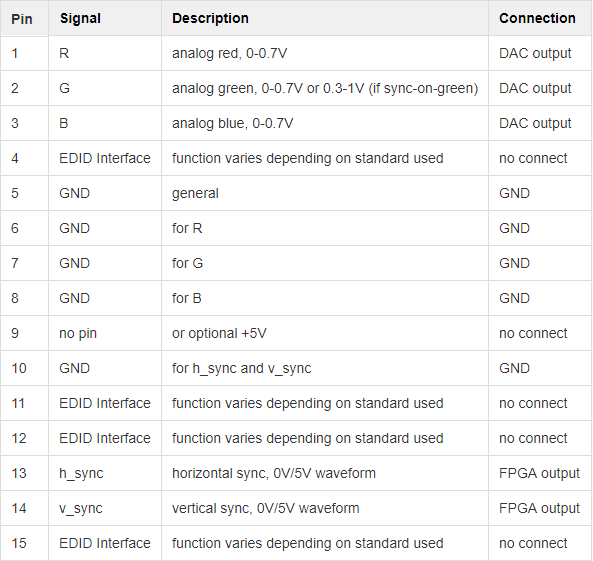
\includegraphics[scale=.5]{figs/vga_pins.png}
    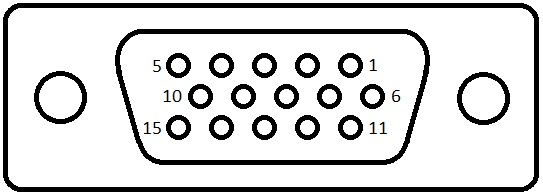
\includegraphics[scale=.5,angle=90]{figs/vga_connector_female.jpg}
}

\frame{
    \frametitle{Temporização}
    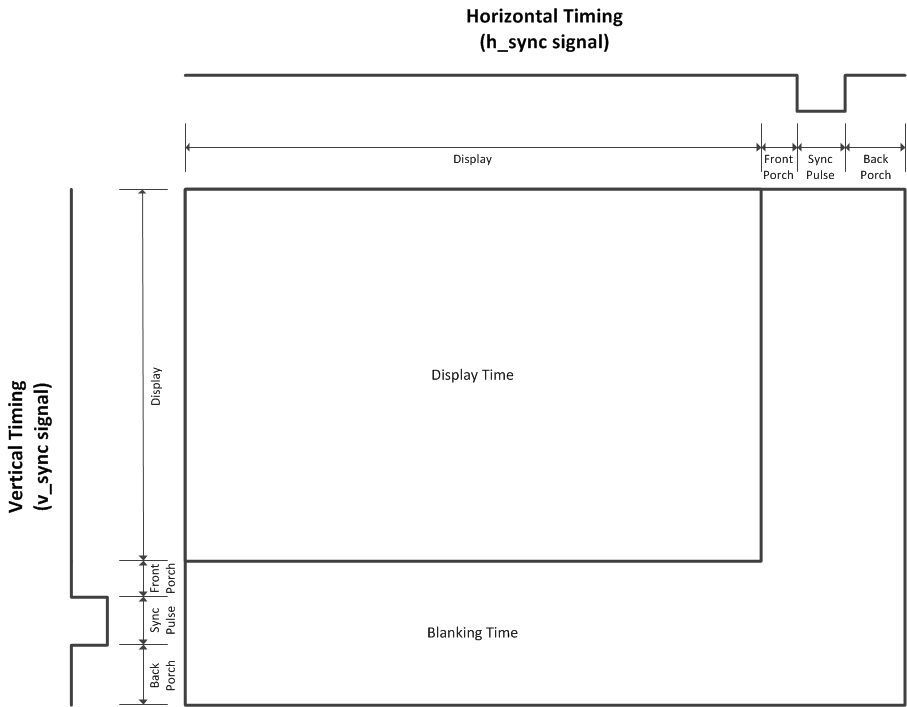
\includegraphics[width=\textwidth]{figs/signal_timing_diagram.jpg}
}

\begin{frame}[fragile]
	\frametitle{Código estático}
	\begin{verilogcode}
module vga640x480(
	input wire dclk,        //pixel clock: 25MHz
	input wire clr,         //asynchronous reset
	output wire hsync,      //horizontal sync out
	output wire vsync,      //vertical sync out
	output reg [3:0] red,   //red vga output
	output reg [3:0] green, //green vga output
	output reg [3:0] blue   //blue vga output
	);	
    \end{verilogcode} 
\end{frame}

\begin{frame}[fragile]
	\frametitle{Código estático}
	\begin{verilogcode}
// video structure constants
parameter hpixels = 800;// horizontal pixels per line
parameter vlines = 521; // vertical lines per frame
parameter hpulse = 96;  // hsync pulse length
parameter vpulse = 2;   // vsync pulse length
parameter hbp = 144;    // end of horizontal back porch
parameter hfp = 784;    // beginning of horizontal front porch
parameter vbp = 31;     // end of vertical back porch
parameter vfp = 511;    // beginning of vertical front porch
// active horizontal video is therefore: 784 - 144 = 640
// active vertical video is therefore: 511 - 31 = 480

// registers for storing the horizontal & vertical counters
reg [9:0] hc;
reg [9:0] vc;
    \end{verilogcode} 
\end{frame}


\begin{frame}[fragile]
	\frametitle{Código estático}
	\begin{verilogcode}
always @(posedge dclk or posedge clr)
begin
  // reset condition
  if (clr == 1) begin
    hc <= 0;
    vc <= 0;
  end
  else begin
    // keep counting until the end of the line
    if (hc < hpixels - 1)
      hc <= hc + 1;
    else begin
    // When we hit the end of the line, reset the horizontal
    // counter and increment the vertical counter.
    // If vertical counter is at the end of the frame, then
    // reset that one too.
      hc <= 0;
      if (vc < vlines - 1)
        vc <= vc + 1;
      else
        vc <= 0;
    end
  end
end
    \end{verilogcode} 
\end{frame}

\begin{frame}[fragile]
	\frametitle{Código estático}
	\begin{verilogcode}
assign hsync = (hc < hpulse) ? 0:1;
assign vsync = (vc < vpulse) ? 0:1;

always @(*)
begin
  // first check if we're within vertical active video range
  if (vc >= vbp && vc < vfp)
  begin
    // now display different colors every 80 pixels
    // while we're within the active horizontal range
    // -----------------
    // display white bar
    if (hc >= hbp && hc < (hbp+80))
    begin
      red   = 4'b1111;
      green = 4'b1111;
      blue  = 4'b1111;
    end
    // display yellow bar
    else if (hc >= (hbp+80) && hc < (hbp+160))
    begin
      red   = 4'b1111;
      green = 4'b1111;
      blue  = 4'b0000;
    ...
    \end{verilogcode} 
\end{frame}



\begin{frame}[fragile]
	\frametitle{Código estático}
	\begin{verilogcode}
	...
    // display black bar
    else if (hc >= (hbp+560) && hc < (hbp+640))
    begin
      red = 4'b0000;
      green = 4'b0000;
      blue = 4'b0000;
    end
    // we're outside active horizontal range so display black
    else
    begin
      red = 0;
      green = 0;
      blue = 0;
    end
  end
  // we're outside active vertical range so display black
  else
  begin
    red = 0;
    green = 0;
    blue = 0;
  end
end
    \end{verilogcode} 
\end{frame}

\section{Integração com o MIPS}

\subsection{Diagrama de blocos} 

\frame{
    \frametitle{Diagrama de blocos}
    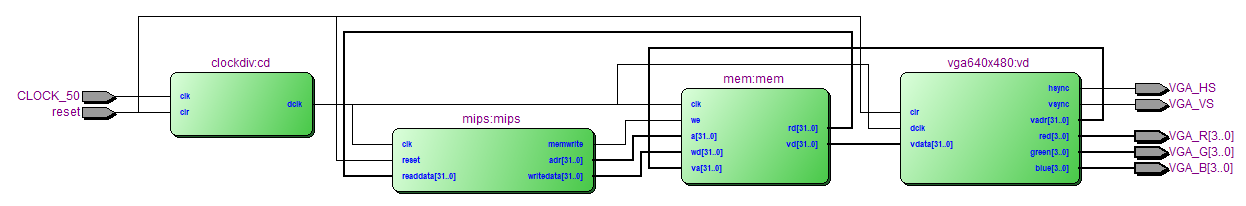
\includegraphics[width=\textwidth]{figs/topmulti}
}

\begin{frame}[fragile]
	\frametitle{Memória com duas portas}
	\begin{verilogcode}
module mem(input  logic        clk, we,
           input  logic [31:0] a, wd, va, 
           output logic [31:0] rd, vd);

  logic  [31:0] RAM[63:0];

  // initialize memory with instructions
  initial
    begin
      $readmemh("memfile.dat", RAM);  
    end

  assign rd = RAM[a[31:2]]; // word aligned

  assign vd = RAM[va[31:2]]; // word aligned

  always_ff @(posedge clk)
    if (we)
      RAM[a[31:2]] <= wd;
endmodule    
    \end{verilogcode} 
\end{frame}

\subsection{Leiaute de Memória} 

\frame{
    \frametitle{Leiaute de Memória}
    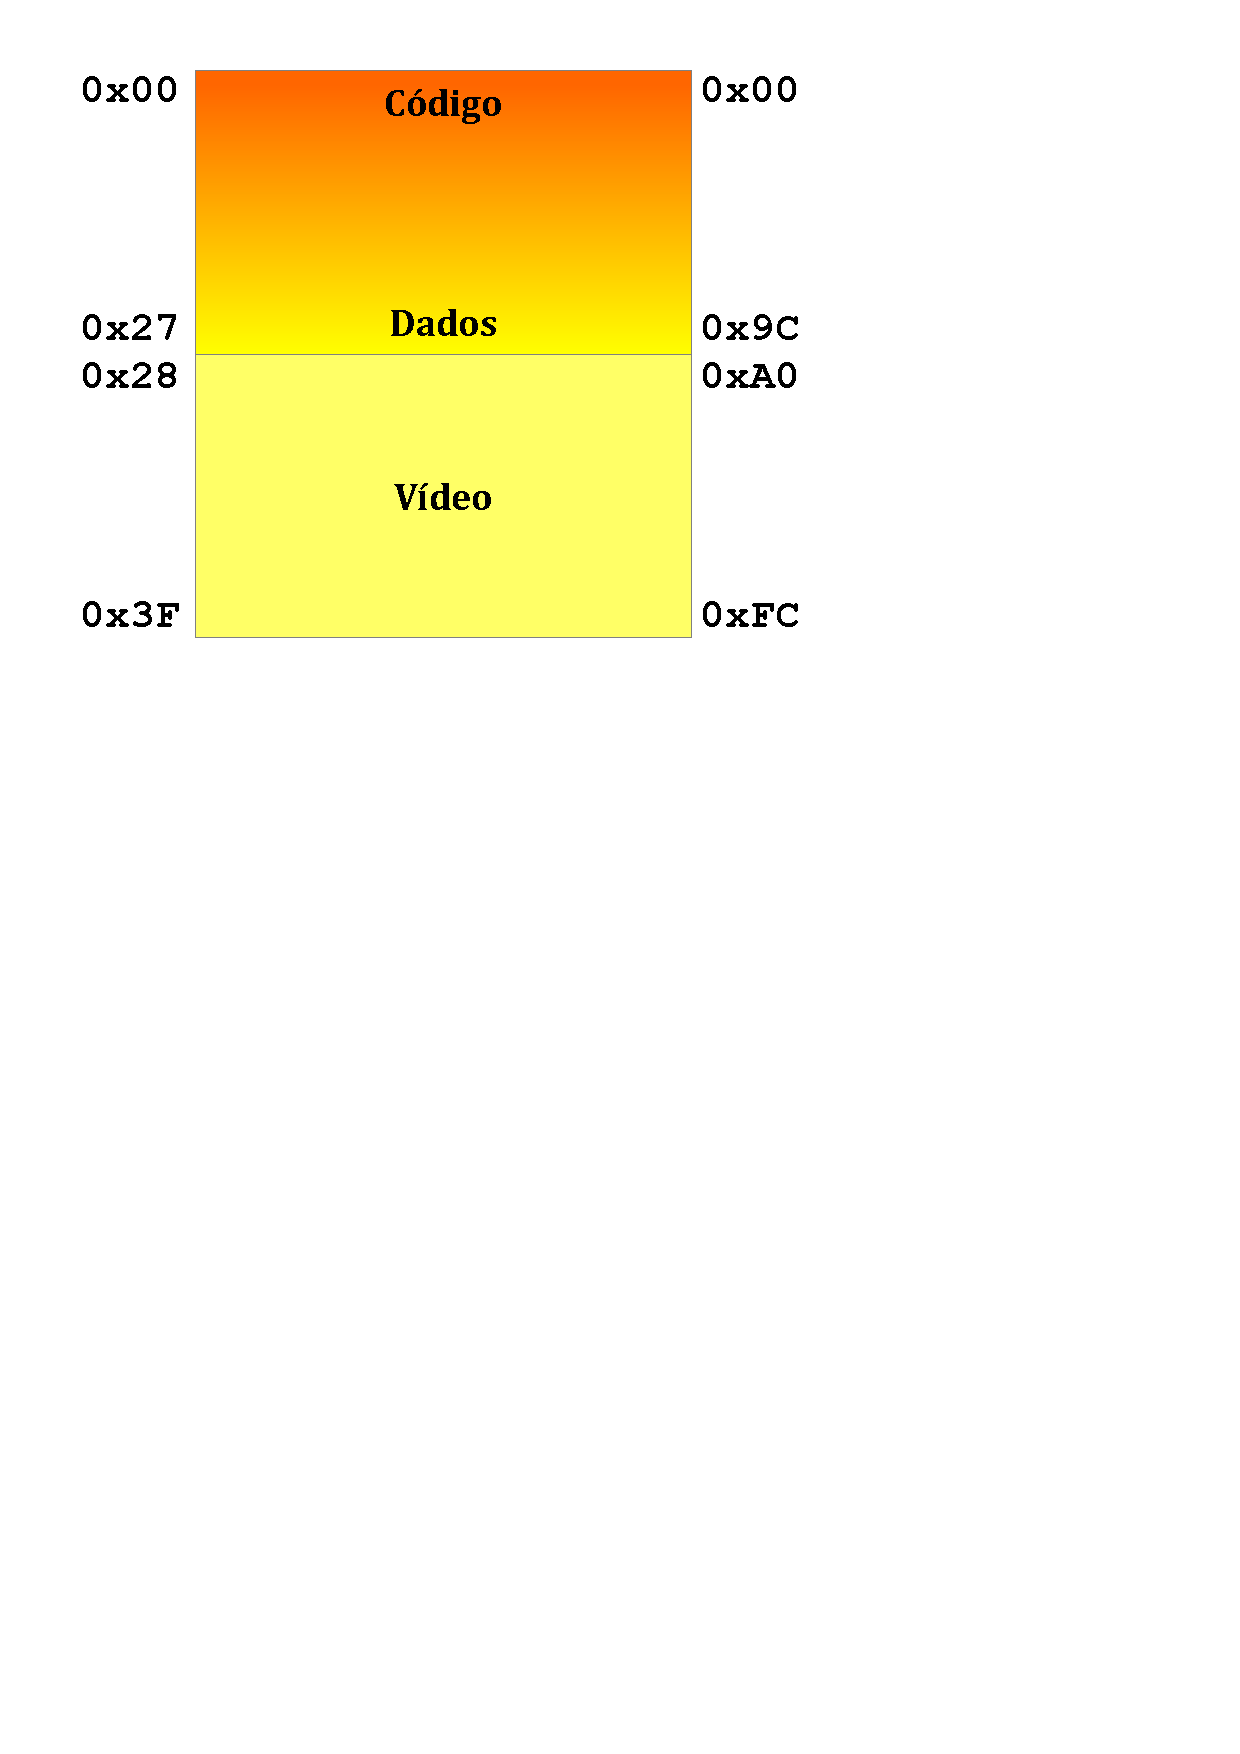
\includegraphics[width=1.4\textwidth]{figs/memleiaute.pdf}
}

\begin{frame}[fragile]
	\frametitle{Código adaptado/corrigido}
	\begin{verilogcode}
module vga640x480(
  input wire dclk,           //pixel clock: 25MHz
  input wire clr,            //asynchronous reset
  input wire [31:0] vdata,   //video data from memory 
  output wire [31:0] vadr,   //video address to memory
  output wire hsync,         //horizontal sync out
  output wire vsync,         //vertical sync out
  output reg [3:0] red,      //red vga output
  output reg [3:0] green,    //green vga output
  output reg [3:0] blue      //blue vga output
  );
    \end{verilogcode} 
\end{frame}

\begin{frame}[fragile]
	\frametitle{Código adaptado/corrigido}
	\begin{verilogcode}
// 480 / 20 = 24 rows  
assign vadr = (vc / 20 + 40)<<2;

// 640 / 20 = 32 columns 
assign pixel = vdata[31-(hc / 20)];

// generate sync pulses (active low)
// ----------------
// "assign" statements are a quick way to
// give values to variables of type: wire
assign hsync = (hc > hpixels-hbp-hpulse && hc < hpixels-hbp) ? 0 : 1;
assign vsync = (vc > vlines-vbp-vpulse && vc < vlines-vbp) ? 0 : 1;
    \end{verilogcode} 
\end{frame}

\begin{frame}[fragile]
	\frametitle{Código adaptado/corrigido}
	\begin{verilogcode}
always @(*)
begin
  // first check if we're within vertical active video range
  if (vc < vlines-vbp-vpulse-vfp)
  begin
    if (hc < hpixels-hbp-hpulse-hfp)
    begin
      red =   {4{pixel}};
      green = {4{pixel}};
      blue = ~{4{pixel}};    
    end
      // we're outside active horizontal range so display black
    else
    begin
      red = 0;
      green = 0;
      blue = 0;
    end
  end
  // we're outside active vertical range so display black
 ...
    \end{verilogcode} 
\end{frame}

\begin{frame}[fragile]
	\frametitle{Programa de teste}
	\begin{nasmcode}
  addi $s1, $zero, 0xfc # final da memoria de video 
loop1:
  addi $s0, $zero, 0xa4 # inicio da memoria de video +1 
loop2:
  lw   $t0, 0($s0)
  addi $t0, $t0, 1
  sw   $t0, 0($s0)
  addi $s0, $s0, 4
  beq  $s0, $s1, loop1
  j loop2    
    \end{nasmcode} 
\end{frame}

\frame{
    \frametitle{Saída inicial}
    \frame{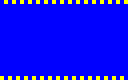
\includegraphics[width=\textwidth]{figs/screen}}
}


\section{Bibliografia} %%%%%%%

\begin{frame}{Bibliografia} 
	\begin{itemize}
        \item \href{https://www.element14.com/community/thread/23394/l/draw-vga-color-bars-with-fpga-in-verilog}{Draw VGA color bars with FPGA in Verilog}
        \item \href{https://eewiki.net/pages/viewpage.action?pageId=15925278}{VGA Controller (VHDL)}
	\end{itemize}
\end{frame}


\begin{frame}
	\titlepage
\end{frame} 

\end{document}
